Эксперименты ставились на парах модельных изображений и на реально отснятых оптических изображениях.

\subsection{Модельные изображения}

В качестве образцов брались наборы изображений из интернет ресурса ``Society for Experimental Mechanics (sem.org)'' несколько видов текстур приведены на рисунках ниже.

\begin{figure}[ht]
\center{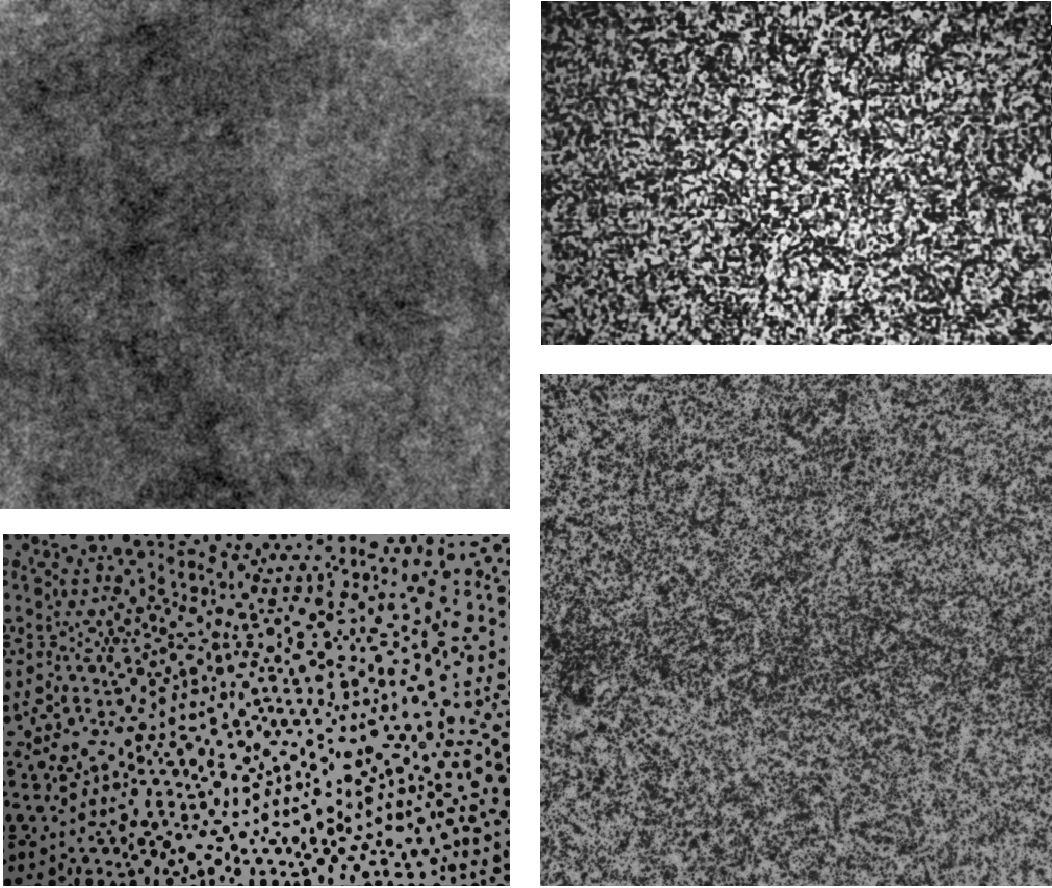
\includegraphics[width=0.8\linewidth]{gray_mix}}
\caption{Тестовая серия изображений: По часовой стрелке Серая подборка, Тестовая серия №11, Серия высокого контраста, Тестовая серия №6}
\label{pic:gray_mix}
\end{figure}

\subsection{Реальные отснятые изображения}

Серия оптических изображений использованных для тестирования программного обеспечения предоставлена Институт физики прочности и материаловедения СО РАН. На серии снимков изображено одноосное растяжение полимерной пластины.

\begin{figure}[ht]
\center{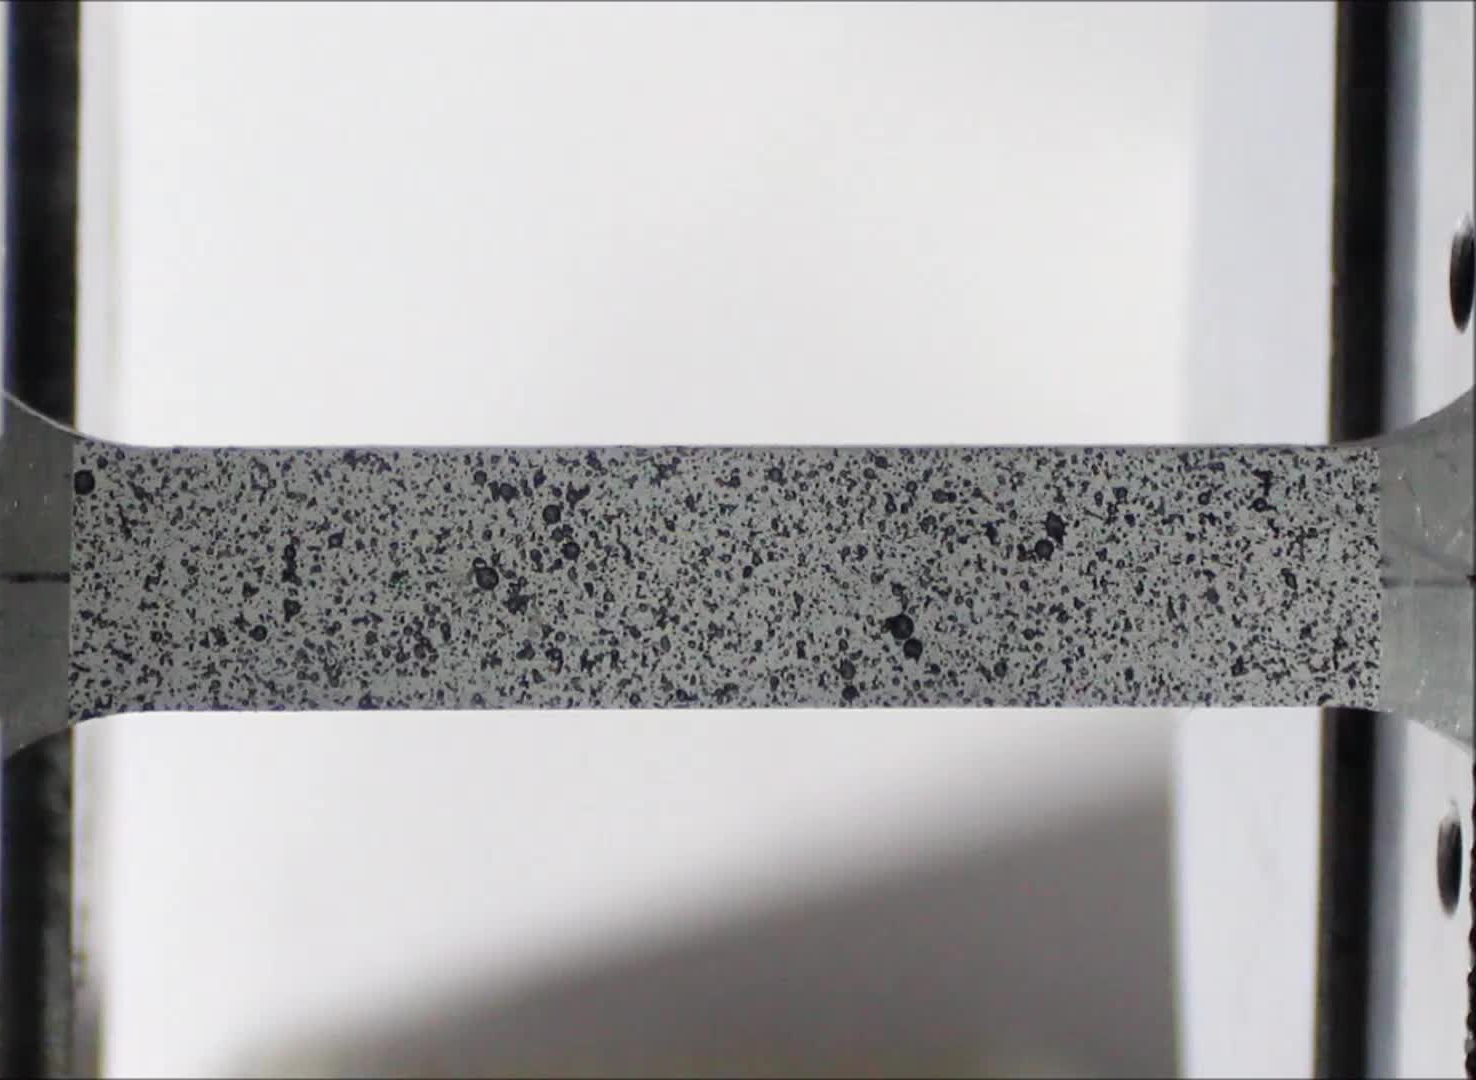
\includegraphics[width=0.6\linewidth]{real_deform}}
\caption{Растяжение пластины алюминия Д16АТ}
\label{pic:real_deform}
\end{figure}
